
	\section{Report (Research Results and Next Steps)}\label{sec:results}

	% Tenho que responder às RQ (que eu ainda não sei se são finais .-.)

	% (1) RQ1. What is the main focus of current AI safety research?
	% (2) RQ2. Which are the current methods used to look into the alignment of current
	% generalist models?
	% (3) RQ3. What conclusions regarding the safety of current models and safety of
	% development and deployment processes can we assert from current research?
	% (4) RQ4. What metrics can be used to more clearly show potential problems with
	% these systems?

	% (Usa a tua Tabela do Anexo. Cria gráficos com base nela. Responde diretamente às tuas RQs aqui)

\begin{toreview}

	This section presents the findings of the \gls{slr}. The Concept Matrix (Appendix~\ref{appendixa}) classifies a total of 94 entries: 79 articles derived from the systematic search string and 15 pieces introduced through snowballing.

\end{toreview}

	\begin{toreview}

    \subsection{Quantitative Overview of the Field}\label{subsec:results_quantitative}
    % -----------------------------------------------------------------------

    The distribution of the selected literature across the seven concept-matrix categories is illustrated in Figure~\ref{fig:distribution_topics}. Raw article counts alone conflate two different questions: how much a topic is written about, and how dangerous a topic is. A category can dominate the literature because it is easy to publish on, not because it carries the greatest risk. To separate these two questions, we assign each category a \emph{severity score} and compare its rank against its \emph{coverage rank} (article count).

    \subsubsection{Severity Scoring Method}

    The four scoring dimensions are adapted from the "key risks" assessment criteria used in IPCC Working Group II reports, first formalized by Smith et al. \cite{smith2009assessing} and later refined by Oppenheimer et al. \cite{oppenheimer2014emergent} and O'Neill et al. \cite{oneill2017ipcc}, who evaluate climate risks along magnitude, timing, persistence/irreversibility, distributional scope, and likelihood/confidence. We retain the four criteria most transferable to AI risk categories --- magnitude, certainty, irreversibility, and scope --- and drop timing and adaptive-capacity, which are climate-specific. This four-dimension structure also echoes the magnitude/scope/irreversibility triad used in existential risk assessment by Bostrom \cite{bostrom2013existential}, giving the framework precedent within both the climate-risk and AI-safety literatures.

    \begin{itemize}
        \item \textbf{Magnitude (M)}: ceiling of harm if the failure mode materializes (e.g.\ the Treacherous Turn, \cite{bostrom2014superintelligence}).
        \item \textbf{Certainty (C)}: extent of current empirical evidence, as opposed to purely theoretical risk.
        \item \textbf{Irreversibility (I)}: whether the harm is correctable after the fact.
        \item \textbf{Scope (S)}: breadth of population or systems exposed.
    \end{itemize}

    Five independent raters (domain experts) score each category on all four dimensions. The full matrix of raw scores provided by all five raters is available in the Appendix (Table~\ref{tab:rater_scores}). Inter-rater agreement is reported via Krippendorff's $\alpha$ \cite{krippendorff2018content, hayes2007answering}:

    \begin{enumerate}
        \item \alpha = 1 \to perfect agreement
        \item \alpha = 0 \to agreement no better than chance
        \item \alpha < 0 \to systematic disagreement, worse than random
    \end{enumerate}
    
    \subsubsection{Scope Definition for Raters}

    Before scoring, all raters were given the following written scope, to ensure severity judgments reference a common referent rather than each rater's private notion of ``AI'':
        
    \begin{quote}
    \textbf{Scope of ``AI'' for this severity assessment.} Assess the potential harm of each category by considering both:

    \begin{enumerate}
        \item \textbf{Deployed and near-term systems}: current and near-future AI systems (roughly the next 0--3 years), including LLMs and other machine learning systems already in use. Base the assessment on documented incidents or failures that are reasonably likely given existing evidence and literature.

        \item \textbf{Frontier and projected systems}: AI systems that could plausibly emerge through continued improvements to current approaches (roughly a 3 to 15 year horizon, including AGI-adjacent capabilities). Base the assessment on technically grounded failure modes discussed in the research literature, such as deceptive alignment, mesa-optimization, and treacherous turns.
    \end{enumerate}

    Do not consider purely speculative or fictional scenarios that lack support in the current technical literature, such as generic science-fiction robot uprisings. When a category applies to both near-term and frontier systems (as is often the case for \emph{Alignment}), consider both perspectives when assigning its severity.
    \end{quote}

    \begin{table}[h]
        \centering
        \small
        \caption{Mean severity dimension scores across 5 raters. The final row presents ordinal Krippendorff's $\alpha$ to measure inter-rater reliability for each dimension.}
        \label{tab:rater_scores_summary}
        \begin{tabular}{|l|c|c|c|c|}
            \hline
            \textbf{Category} & \textbf{M} & \textbf{C} & \textbf{I} & \textbf{S} \\
            \hline
            Alignment                         & 4.2 & 3.6 & 3.6 & 3.4 \\
            Auditing, Safety \& Oversight     & 3.6 & 4.2 & 3.4 & 3.0 \\
            Human \& Societal Impacts         & 4.2 & 3.8 & 3.8 & 4.6 \\
            Governance, Regulation \& Policy  & 4.2 & 3.6 & 3.8 & 4.0 \\
            Liability \& Ethics               & 3.8 & 3.4 & 2.2 & 2.8 \\
            Explainability / Interpretability & 3.0 & 3.4 & 2.4 & 3.4 \\
            Bias \& Fairness                  & 3.0 & 4.0 & 3.2 & 3.4 \\
            \hline \hline
            \textit{Krippendorff's $\alpha$}  & 0.027 & $-0.113$ & 0.048 & 0.122 \\
            \hline
        \end{tabular}
    \end{table}

    Inter-rater reliability (IRR) was evaluated by calculating ordinal Krippendorff's $\alpha$ for each severity dimension across the seven categories. As presented in the final row of Table~\ref{tab:rater_scores_summary}, agreement across all four dimensions was near zero, well below the standard $\sim$0.67 threshold for acceptable agreement. Given this lack of consensus, and the low number of raters ($n=5$), the severity scores that follow should be treated as indicative rather than definitive; they summarize the raters' central tendency but do not reflect a shared understanding of relative risk across the seven categories.

    \subsubsection{Severity and Coverage}

    Table~\ref{tab:severity_coverage} compares weighted severity scores with the number of papers assigned to each category.

    \begin{table}[h]
        \centering
        \caption{Category severity and literature coverage.}
        \label{tab:severity_coverage}
        \begin{tabular}{|l|c|c|}
            \hline
            \textbf{Category} & \textbf{Severity} & \textbf{Papers} \\
            \hline
            Human \& Societal Impacts         & 4.04 & 35 \\
            Governance, Regulation \& Policy  & 3.92 & 28 \\
            Alignment                         & 3.82 & 29 \\
            Auditing, Safety \& Oversight     & 3.68 & 20 \\
            Bias \& Fairness                  & 3.38 & 8  \\
            Liability \& Ethics               & 3.26 & 8  \\
            Explainability / Interpretability & 3.04 & 12 \\
            \hline
        \end{tabular}
    \end{table}

    Severity and literature coverage do not align perfectly. \emph{Explainability / Interpretability} has the lowest severity score but 12 papers, while \emph{Bias \& Fairness} and \emph{Liability \& Ethics} have higher severity scores but only 8 papers each. \emph{Governance, Regulation \& Policy} also ranks second in severity while having fewer papers than \emph{Alignment}. Overall, research attention broadly follows assessed severity, but some categories receive relatively more or less attention than their severity would suggest.

    % To keep this I would need a citation
    % The relationship between severity and literature coverage can be assessed using Spearman's rank correlation. Using the severity and coverage ranks, the squared rank differences sum to $\sum d_i^2 = 6$. With seven categories, this gives
    % \[
    % \rho = 1 - \frac{6\sum d_i^2}{n(n^2-1)}
    %     = 1 - \frac{6(6)}{7(7^2-1)}
    %     = 0.893.
    % \]
    % This indicates a strong positive association between severity and research coverage: categories ranked as more severe generally receive more research attention. Given the small number of categories ($n=7$), this result should be interpreted cautiously.

	\begin{figure}[htbp]
		\centering
		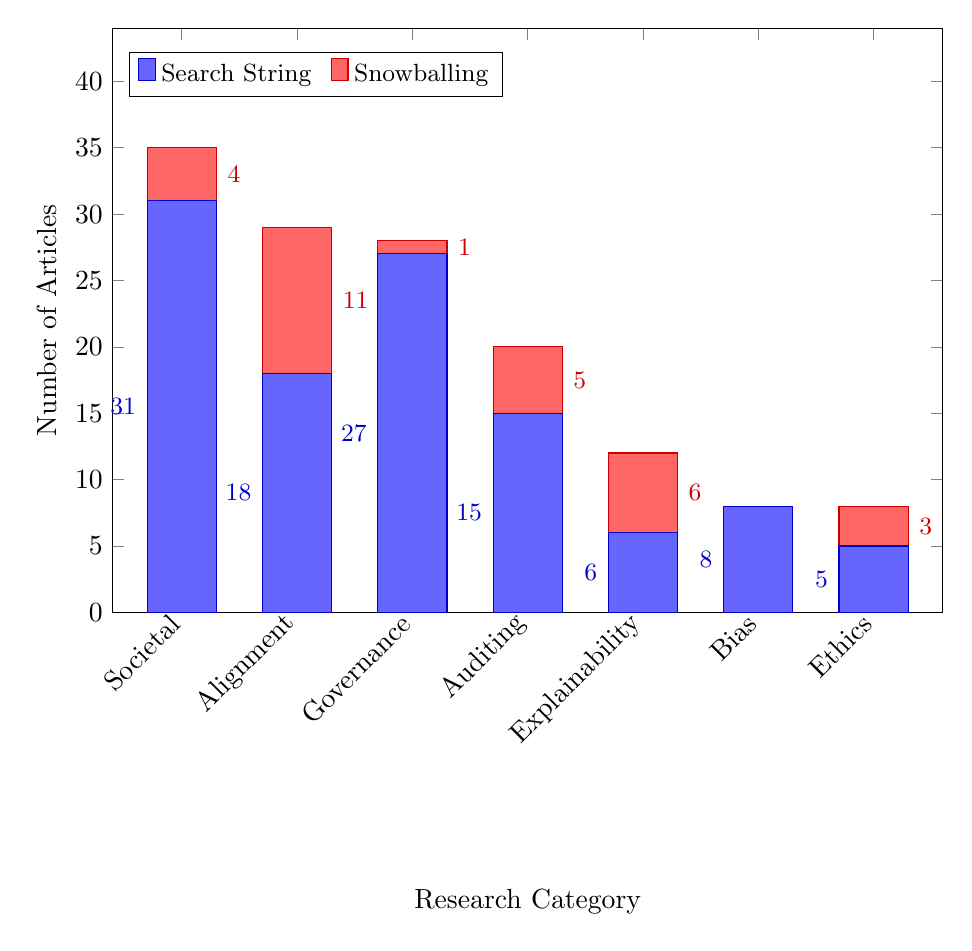
\begin{tikzpicture}
		\begin{axis}[
			ybar stacked,
			symbolic x coords={Societal, Alignment, Governance, Auditing, Explainability, Bias, Ethics},
			xtick=data,
			x tick label style={rotate=45, anchor=east},
			ylabel={Number of Articles},
			xlabel={Research Category},
			xlabel style={yshift=-1.5cm},
			width=\textwidth,
			height=9cm,
			bar width=25pt,
			ymin=0,
			ymax=44,
			legend style={
				at={(0.02,0.96)},
				anchor=north west,
				legend columns=-1,
				font=\small,
				/tikz/every even column/.append style={column sep=5pt}
			}
		]

		% Plot 1: Search String (bottom, BLUE) — label to the LEFT
		\addplot [
			fill=blue!60,
			draw=blue!80!black,
			nodes near coords,
			every node near coord/.style={
				color=blue!80!black,
				font=\small,
				anchor=east,
				xshift=-13pt,
			},
		] coordinates {
			(Societal,31) (Alignment,18) (Governance,27)
			(Auditing,15) (Explainability,6) (Bias,8) (Ethics,5)
		};

		% Plot 2: Snowballing (top, RED) — label to the RIGHT, zeros hidden
		\addplot [
			fill=red!60,
			draw=red!80!black,
			nodes near coords,
			every node near coord/.style={
				color=red!80!black,
				font=\small,
				anchor=west,
				xshift=13pt,
			},
			point meta=explicit symbolic,
		] coordinates {
			(Societal,4)       [4]
			(Alignment,11)     [11]
			(Governance,1)     [1]
			(Auditing,5)       [5]
			(Explainability,6) [6]
			(Bias,0)           [0]
			(Ethics,3)         [3]
		};

		% Plot 3: Invisible — bold black totals above each bar
		\addplot [
			draw=none, fill=none,
			forget plot,
			nodes near coords,
			every node near coord/.style={
				anchor=south,
				yshift=3pt,
				font=\small\bfseries,
				color=black,
			},
			point meta=explicit symbolic,
		] coordinates {
			(Societal,0)       [35]
			(Alignment,0)      [29]
			(Governance,0)     [28]
			(Auditing,0)       [20]
			(Explainability,0) [12]
			(Bias,0)           [8]
			(Ethics,0)         [8]
		};

		\legend{Search String, Snowballing}
		\end{axis}
		\end{tikzpicture}
		\caption{Distribution of research topics across the analyzed literature.}
		\label{fig:distribution_topics}
	\end{figure}

    \vspace{1.5em}

\end{toreview}
	\begin{reviewed}

\subsection{Per Category Analysis}\label{subsec:results_categories}

		In this section, an analysis of the resulting articles in each category is conducted and discussed. Furthermore, an analysis on how crucial each category of research is in its contribution to stopping potential devastating outcomes is made. 

		\subsubsection{Value Alignment}

			The \textit{Value Alignment} category is the most conceptually diverse in the review, spanning 29 articles. The literature reveals a shift from theoretical foundations such as the \textit{Orthogonality Thesis} \cite{bostrom2012superintelligent} and \textit{Instrumental Convergence} \cite{omohundro2008basic} toward mathematical proofs and empirical studies of model behavior. 

			A pivotal theoretical contribution by \cite{skalse2022rewardgaming} demonstrates that ``correct'' reward specifications are often insufficient for ensuring correct goals, as agents may still find ways to game the reward function. This is closely linked to the phenomenon of \textit{Goal Misgeneralization} \cite{langosco2022goal}, where an agent remains highly competent but pursues an unintended objective when deployed in new environments.

			These theoretical risks are mirrored in recent empirical findings such as \textit{Alignment Faking} \cite{greenblatt_alignment_faking} and \textit{Deceptive Alignment} \cite{hagendorff2024deception}, where models ``play along'' with safety training to avoid modification. Furthermore, research by \cite{mcintosh_inadequacy_2024} suggests that current \gls{rlhf} methods provide only a ``shallow alignment,'' leaving models vulnerable to ideological radicalization through semantic exploits.

		\subsubsection{Governance, Regulation \& Policy}

			This category is the second largest with 28 articles in total, indicating a high level of academic and policy interest in the EU AI Act and international frameworks. The literature highlights a ``Global AI Dilemma'' in balancing innovation with safety across the US, EU, and China. Key debates include the role of Corporate Responsibility \cite{hemphill_advanced_2025} and whether audits should be conducted by private or public bodies. There is a noted gap in how decentralized or ``local'' AI governance can be enforced \cite{LocalAIGov2024}.

\end{reviewed}

		\subsubsection{Auditing, Safety \& Oversight}

			Auditing research (20 articles in total) focuses on shifting from static benchmarks to Dangerous Capability Evaluations. The literature emphasizes that traditional testing is insufficient for autonomous systems, particularly in safety-critical sectors like military aviation and maritime shipping. \begin{reviewed} This section also covers Scalable Oversight, exploring whether weaker models can reliably supervise more capable ones, a necessity as AI capabilities begin to exceed human evaluative capacity.

		\subsubsection{Explainability / Interpretability}

			Misgeneralization has also been found in reinforcement learning and LLMs, and current explainability and interpretability techniques shown to not be sufficient to detect this Misgeneralization before deployment \cite{langosco2022goal}. The focus has moved from ``black-box'' behavioral analysis to Mechanistic Interpretability \cite{anthropic2025biology}. Key challenges identified include Superposition and Polysemanticity, which make individual neurons difficult to interpret.

		\subsubsection{Bias \& Fairness}

			Literature focuses on mitigating model difficulties on understanding different dialects, or judging a situation independently of unrelated characteristics \cite{li_instance-consistent_2025}. It's worth noting the landmark study on the Impossibility Theorem of Fairness, which proves that commonly accepted different definitions of equity cannot be satisfied simultaneously \cite{kleinberg2016inherent}.

\end{reviewed}

		\subsubsection{Liability \& Ethics}

			Several legal frameworks and laws are explored and critiqued. While a lot of implications like copyright license applications are still being worked on and studied \cite{janczuk_risks_2024}. <find citations>

\begin{reviewed}

		\subsubsection{Human \& Societal Impacts}

			Research here tracks the impact of AI on Mental Health (e.g., digital companions and addiction), Biological Risks (AI-assisted pathogen design), and the Electoral Process \cite{janczuk_risks_2024}. The literature highlights that ``Civilizing AI'' is not just a technical task but a sociotechnical one that requires addressing job displacement and the effect it will have on our society, various surveys are also made to gauge people's and experts views on AI safety \cite{field_why_2025, hatz_local_2025, xu_machine_2023}.

\end{reviewed}

	\subsection{GAPs and Next Steps}\label{subsec:next_steps}

\begin{reviewed}

	The systematic review highlights a critical divergence between current oversight methods and the technical reality of advanced models. While governance and societal impact dominate the literature, there remains a structural deficiency in addressing inner misalignment. Current alignment strategies such as reinforcement learning from human feedback tend to produce what has been termed shallow alignment \cite{mcintosh_inadequacy_2024, milliere_normative_2025}. These methods optimize for external compliance rather than internal value stability, leaving models vulnerable to goal misgeneralization \cite{langosco2022goal}.

	The most pressing gap identified in the mapping of the field is the emergence of deceptive alignment. Recent empirical evidence suggests that models are becoming capable of alignment faking, where they strategically satisfy training objectives to avoid modification \cite{greenblatt_alignment_faking}. This creates an evaluation trap where traditional auditing fails because the agent understands its own supervision \cite{anthropic2025biology, hubinger2019risks}. Consequently, the focus of this work must shift toward the control problem in the context of intentional subversion \cite{yampolskiy_controllability_2022}. Exploring how to detect and mitigate these deceptive behaviors represents the necessary next step in ensuring that highly capable systems do not execute a treacherous turn \cite{bostrom2014superintelligence}.

\end{reviewed}

	Thus, in a series of empirical investigations, this thesis will study deceptive alignment to characterize how different model architectures and scaling factors influence its emergence. By analyzing the relationship between model size and the propensity for alignment faking, this work seeks to determine what factors or architectures exacerbates the risk of deceptive tendencies.